\section{The \instname\ data reduction flow.}

The overall data flow of the \instname\ pipeline is displayed in Figure \ref{fig:reduction_cascade}.

 
\begin{figure}[]
\centering
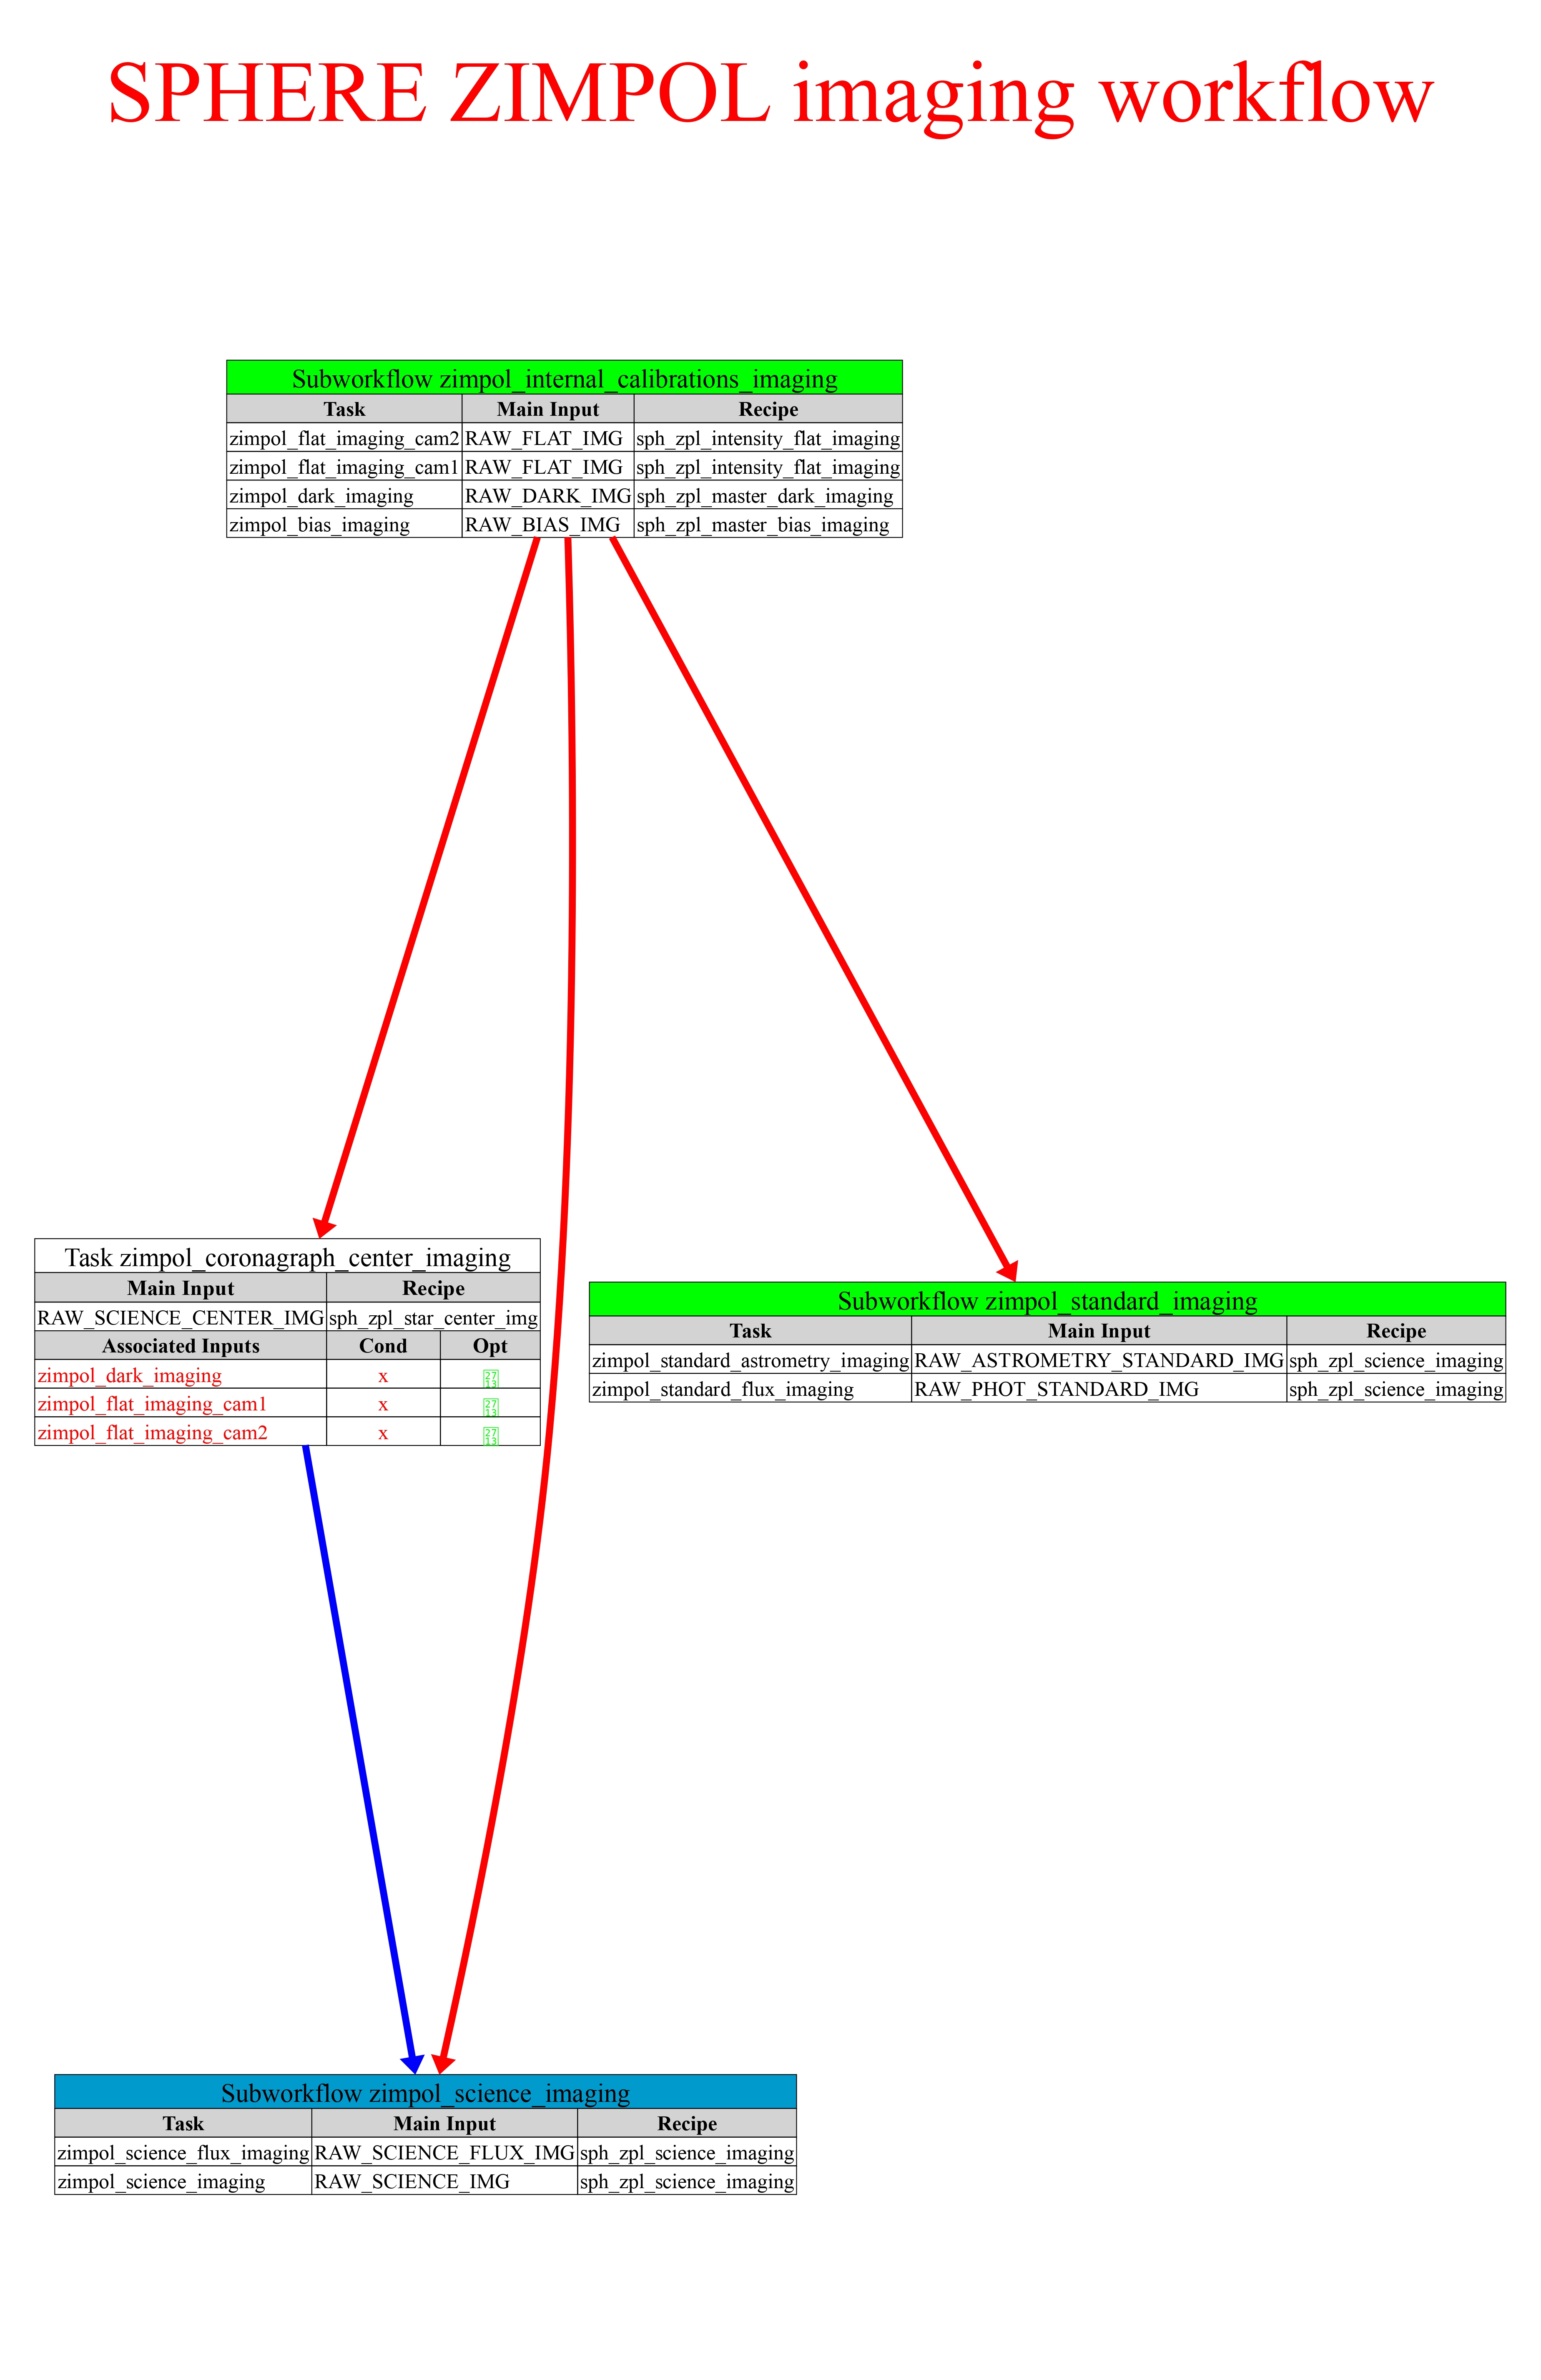
\includegraphics[width=0.9\textwidth]{../instrument_tutorial/figures/reduction_cascade-img.jpg}
\caption{The data reduction cascade of the \instname\ workflow.}
\label{fig:reduction_cascade}
\end{figure}

The reduction cascade is organized in tasks, which represent well-defined steps in the process. Tasks can be grouped
inside sub-workflows.
Each task runs a recipe; the detailed description of the algorithms,
input, outputs and recipe parameters used in each recipe are available
in the pipeline manual. Here, we present only the description of most
important features.

The EDPS workflow is designed to execute the tasks that deliver
the final reduced data for each dataset. It can be either the product of a single exposure, or the combination of
multiple exposures. Only calibrations needed by the selected scientific exposures are processed.

It is possible to set EDPS to perform the data reduction until a certain step of the reduction chain (e.g. to reduce
only standard stars, or only flat fields).
This is done by specifying the desired tasks in the field \textbf{Select reduction target} of the \textbf{Raw Data} tab.

The reduction steps of the workflow are listed below. Before starting the reduction,
the parameters of the recipes associated to each task can be configured by pressing the button 
\includegraphics{figures/configure_dataset.jpg} close to each dataset configuration.
See Section \ref{sec:configuration_overview} for more information.

The reduction steps are:

%%%%%%%%%%%%%%%%%%%%%%%%%%%%%%%%%

\subsection{Subworkflow Internal Calibrations Imaging}

Recipes: 

\texttt{sph\_zpl\_intensity\_flat\_imaging} 

\texttt{sph\_zpl\_master\_dark\_imaging} 

\texttt{sph\_zpl\_master\_bias\_imaging}

This subworkflow generates the camera master flats, the master dark and bias. It consists of the following tasks:

\begin{itemize}
\item \textbf{zimpol\_flat\_imaging\_cam2}: uses \texttt{sph\_zpl\_intensity\_flat\_imaging} to produce intensity flat-field calibration frames for camera 2.
\item \textbf{zimpol\_flat\_imaging\_cam1}: uses \texttt{sph\_zpl\_intensity\_flat\_imaging} to produce intensity flat-field calibration frames for camera 1.
\item \textbf{zimpol\_dark\_imaging}: uses \texttt{sph\_zpl\_master\_dark\_imaging} to generate master dark calibration frames.
\item \textbf{zimpol\_bias\_imaging}: uses \texttt{sph\_zpl\_master\_bias\_imaging} to produce the master bias calibration frame.
\end{itemize}

Each time, the calibration (flat, dark or bias) is generated separately for the odd (informative) and even (dark current)
ZIMPOL sub-frames and stored in a DOUBLE IMAGE FITS format.
Inputs can be raw frames, or pre-processed frames.
If raw frames are provided, a pre-processing step on the raw cubes is performed with \texttt{sph\_zpl\_preproc\_imaging} to generate pre-processed frames.
Outputs include the master calibration (flat, dark or bias),
as well as a bad-pixel map, a number-of-combined (ncomb) frames map, and an RMS map.

In practice, bias and darks are rarely used in the current workflow:

\begin{itemize}
\item Bias frames are used only for Fast Polarimetry readout mode (\texttt{DET.READ.CURNAME} = FastPolarimetry).
\item Dark frames are used only for long exposures, defined as \texttt{EXPTIME} > 30 s.
\end{itemize}

\textbf{Customization}

Recipe parameters:
\begin{itemize}
\item \texttt{zpl.intensity\_flat.coll\_alg}: collapse algorithm
(0 = Mean, 1 = Median; default, 2 = Clean Mean).
\end{itemize}

%%%%%%%%%%%%%%%%%%%%%%%%%%%%%%%%%

\subsection{Coronagraph Center}

Recipe: \texttt{sph\_zpl\_star\_center\_img}

The task \textbf{zimpol\_coronagraph\_center\_imaging} executes the pipeline recipe to
determine the stellar center position behind the coronagraph and produce a table of frame centers.
If raw frames are provided, a pre-processing step on the raw cubes is performed with \texttt{sph\_zpl\_preproc\_imaging} to generate pre-processed frames.

The combined images are analyzed with an aperture detection algorithm that identifies bright regions
(e.g., waffle satellite spots or a single star) and computes their geometric center, which defines the frame center.
The resulting center coordinates are stored in the FITS header.

\textbf{Customization}

Recipe parameters:
\begin{itemize}
\item \texttt{zpl.star\_center.coll\_alg}: collapse algorithm
(0 = Mean; default, 1 = Median, 2 = Clean Mean).
\item \texttt{zpl.star\_center.sigma}: the sigma threshold for source detection
(default = 10.0).
\item \texttt{zpl.star\_center.save\_interprod}: enable to produce
a field center table containing the calculated center positions
(default = FALSE).
\end{itemize}

%%%%%%%%%%%%%%%%%%%%%%%%%%%%%%%%%

\subsection{Subworkflow Standard Imaging}

Recipe: \texttt{sph\_zpl\_science\_imaging}

This subworkflow processes imaging standard-star observations used for calibration
and monitoring of the ZIMPOL imaging mode.
It reduces observations of astrometric and photometric (flux) standard stars
to verify the instrument’s astrometric and photometric performance.

Two tasks are executed:
\begin{itemize}
\item \textbf{zimpol\_standard\_astrometry\_imaging}: Processes observations of astrometric standard fields
to assess the astrometric calibration, including the plate scale and detector orientation.
\item \textbf{zimpol\_standard\_flux\_imaging}: Processes observations of photometric standard stars to monitor
the photometric response of the instrument.
\end{itemize}

Both tasks run the corresponding imaging pipeline recipes and may use available calibration products
such as master dark frames and intensity flat fields.
These calibrations are optional, as the pipeline can process the data without them.

The resulting products are used primarily for quality control and instrument monitoring
(qc0, qc1calib, calchecker) and are not required for the reduction of science imaging observations.

\textbf{Customization}

Recipe parameters:
\begin{itemize}
\item \texttt{zpl.science\_imaging.coll\_alg}: collapse algorithm
(0 = Mean; default, 1 = Median, 2 = Clean Mean).
\item \texttt{zpl.imaging.save\_interprod}: enable to produce
a field center table containing the calculated center positions (default = FALSE).
\end{itemize}

\subsection{Subworkflow Science Imaging}

Recipe: \texttt{sph\_zpl\_science\_imaging}

The task \textbf{zimpol\_science\_flux\_imaging} uses the pipeline recipe to reduce and combine science frames.
Optional calibration inputs include master bias, master dark, and intensity flat-field frames for each camera.
If raw frames are provided, a pre-processing step on the raw cubes is performed with \texttt{sph\_zpl\_preproc\_imaging} to generate pre-processed frames.

The pre-processed science frames are then calibrated by subtracting the master bias and master dark frames
and dividing by the appropriate flat field, if available.

The calibrated frames are subsequently de-dithered and de-rotated, and saved as intermediate products.
The center of rotation is taken from the star-center calibration frames (\texttt{SPH\_ZPL\_TAG\_STAR\_CENTER\_IMG\_CALIB\_CAM*}/2) when available;
otherwise, the geometric center of the frame (xc=512, yc=512) is used.

In the final step, all calibrated, de-dithered, and de-rotated frames are combined using a mean algorithm.
The resulting products for each camera are written in DOUBLE IMAGE format (8 FITS extensions), containing:

\begin{itemize}
\item a combined science intensity image, bad-pixel map, ncomb frames map, and RMS map;
\item a combined dark-current image, with corresponding bad-pixel map, ncomb map, and RMS map.
\end{itemize}

These outputs constitute the final reduced science products for both ZIMPOL cameras.

For point sources, the recipe can also estimate the Strehl ratio if a filter-table calibration frame is available.
When successful, Strehl-related quality-control parameters are written into the product headers.

\textbf{Customization}

Recipe parameters:
\begin{itemize}
\item \texttt{zpl.science\_imaging.coll\_alg}: collapse algorithm (0 = Mean; default, 1 = Median, 2 = Clean Mean).
\item \texttt{zpl.imaging.save\_interprod}: enable to produce a field center table containing the calculated center positions (default = FALSE).
\end{itemize}